\section{Semantics of Communicating Processes}
In this section, first, we define a simple language
and we define the event structure semantics of this language.

% \subsection{Normal }

Let $\mc{A}$ be the set of possible labels for event structures.
We define a language with the following syntax:

\begin{align*}
    p ::= nil ~|~ \alpha p ~|~ p_0 + p_1 ~|~ p_0 \times p_1
    ~|~ p\lceil \Lambda
\end{align*}

where $\alpha \in \mc{A}$ and $\Lambda \subseteq \mc{A}$.

\subsection{Denotational Semantics}

\begin{definition}
    We define the semantic map $\sem{ \ }: p \ra \mathbb{E}$ where
    $\mathbb{E}$ is the set of all event structures with
    labels in $\mc{A}$ as follows:
    \begin{align*}
        \sem{nil}      & = (\emptyset,\emptyset)                  \\
        \sem{\alpha t} & = \alpha\sem{t}                        \\
        \sem{t_1 + t_2}
                        & = \sem{t_1} + \sem{t_2}                  \\
        \sem{t \lceil \Lambda}
                        & = \sem{t} \lceil \Lambda \\
        \sem{t_1 \times t_2}
                        & = \sem{t_1} \times \sem{t_2}
    \end{align*}
\end{definition}

\subsection{Examples}
In the following, we provide some examples to illustrate
how the prefix, sum, and product operators can be used to 
compose event structures.
For simplicity, assume that $ \mc{A} = \s{a,b,c}$. 

\begin{example}
    $\mr{E} = \sem{ab}$ is an event structure
    $(E,\#,\vdash,L,l)$ where:
    \begin{align*}
        E  & = \s{(0,a),(1,0,b)}                       \\
        \# & = \emptyset                               \\
           & \e \vdash (0,a), \s{(0,a)} \vdash (1,0,b) \\
        L  & = \s{a,b}                                 \\
           & l((0,a)) = a, l((1,0,b)) = b              
    \end{align*}
    The following diagram shows configurations of $\mr{E}$:
    \begin{center}
        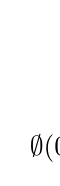
\begin{tikzpicture}[scale=0.8]
            \crd[right]{0}{0}{$\emptyset$}
            \crd[right]{0}{1}{$\s{(0,a)}$}
            \crd[right]{0}{2}{$\s{(0,a),(1,0,b)}$}
            \draw [ultra thick] (0,0) -- (0,1);
            \draw [ultra thick] (0,1) -- (0,2);
        \end{tikzpicture}
    \end{center}
\end{example}

\begin{example}
    $\mr{E} = \sem{a + b}$ is an event structure
    $(E,\#,\vdash,L,l)$ where:
    \begin{align*}
        E & = \s{(0,a),(1,b)}                \\
          & (0,a) \# (1,b)   \\
          & \e \vdash (0,a), \e \vdash (1,b) \\
        L & = \s{a,b}                        \\
          & l((0,a)) = a, l((1,b)) = b       
    \end{align*}
    The following diagram shows configurations of $\mr{E}$:
    \begin{center}
        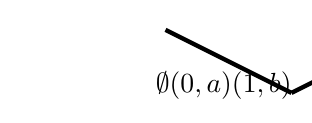
\begin{tikzpicture}[scale=0.8]
            \crd[above]{0}{0}{$\emptyset$}
            \crd[above]{-2}{1}{$\s{(0,a)}$}
            \crd[above]{2}{1}{$\s{(1,b)}$}
            \draw [ultra thick] (0,0) -- (-2,1);
            \draw [ultra thick] (0,0) -- (2,1);
        \end{tikzpicture}
    \end{center}
\end{example}


\begin{example}
    $\mr{E} = \sem{a \times b}$ is an event structure
    $(E,\#,\vdash,L,l)$ where:
    \begin{align*}
        E  & = \s{(a,*),(*,b),(a,b)}                           \\
        \# & = \e                                              \\
           & \e \vdash (a,*), \e \vdash (*,b),\e \vdash (a,b)  \\
        L  & = \s{(a,*),(*,b),(a,b)}                           \\
           & l((a,*)) = (a,*), l((*,b)) = (*,b),l((a,b))=(a,b) 
    \end{align*}
    The following diagram shows configurations of $\mr{E}$:
    \begin{center}
        \begin{tikzpicture}[scale=0.8]
            \crd[above]{0}{0}{$\emptyset$}
            \crd[left]{-2}{1}{$\s{(a,*)}$}
            \crd[right]{2}{1}{$\s{(*,b)}$}
            \crd[above]{0}{2}{$\s{(a,*),(*,b)}$}
            \crd[above]{2}{3}{$\s{(a,b)}$}
            \draw [ultra thick] (0,0) -- (-2,1);
            \draw [ultra thick] (0,0) -- (2,1);
            \draw [ultra thick] (2,1) -- (0,2);
            \draw [ultra thick] (-2,1) -- (0,2);
            \draw [ultra thick] (0,0) -- (2,3);
        \end{tikzpicture}
    \end{center}
\end{example}